\documentclass[aspectratio=169,usenames,dvipsnames]{beamer}
\beamertemplatenavigationsymbolsempty
% \documentclass{beamer}

% UNCOMMENT FOR HANDOUTS
% \usepackage{pgfpages}
% \pgfpagesuselayout{2 on 1}[landscape,letterpaper,border shrink=5mm]
% \setbeameroption{show notes}

\mode<presentation>
\usetheme{Boadilla}
\usecolortheme{spruce}
\usepackage{../LizStyle,ulem}
\usepackage{color}
\usepackage[color,matrix,arrow]{xy}
% \input xy
% \xyoption{all}
\usepackage{tikz}
\usepackage{tikz-cd}
\tikzset{commutative diagrams/diagrams={ampersand replacement=\&}}

\AtBeginSection{\frame{\sectionpage}}


% ==========Command for putting comments and removing them=======
% Visible:
\newcommand{\InstructorNotes}[1]{\textit{\color{orange}#1}}
\newcommand{\InstructorList}[1]{
\begin{itemize}
	\color{orange}
	#1
\end{itemize}
}
% Removed:
% \renewcommand{\InstructorNotes}[1]{}
% \renewcommand{\InstructorList}[1]{}


\newcommand{\bvfill}{\vskip0pt plus 1filll}

\usepackage{multimedia}
\usepackage{graphbox}

% \usepackage{algpseudocode}


\newcommand{\Reeb}{\textbf{Reeb}}
\newcommand{\Rtopc}{\textbf{Rtopc}}
% \newcommand{\RR}{\mathcal{R}}

\newcommand{\Set}{\textbf{Set}}
\newcommand{\Vect}{\textbf{Vect}}
\newcommand{\Top}{\textbf{Top}}
\newcommand{\Int}{\textbf{Int}}


\graphicspath{ {Figures/} {../Figures/}{../../Figures/} }



\begin{document}
%\pdfoptionpdfminorversion 5
%\logo{\includegraphics[height=1.5cm]{dukeshield.pdf}}
\title[]{Ch 6.3, 6.4: PLS; Curse of Dimensionality}
\subtitle{Lecture 21 - CMSE 381}
\date{Mon, Oct 30, 2023}



\institute[MSU-CMSE]{Michigan State University\\
			::\\
          Dept of Computational Mathematics, Science \& Engineering}
\author[Dr.~Munch]{Prof.~Elizabeth Munch}

\begin{frame}
 \titlepage


\end{frame}
%--------------------------
\begin{frame}[c]{Announcements}

\begin{columns}
\column{.45\textwidth}
\centering

	\textbf{Last time:}
	\begin{itemize}
		\item PCA/PCR
	\end{itemize}

	\vspace{.2in}

	\textbf{This lecture:}
	\begin{itemize}
	\item Finish PCR
	\item 6.3: PLS
	\item 6.4: Issues with higher dimensions
\end{itemize}


\column{.45\textwidth}
\centering

\textbf{Announcements:}
	\begin{itemize}
		\item Homework \#5 due Friday 

	\end{itemize}
\end{columns}

\end{frame}
%--- Next Frame ---%



%=================
\section{Last time}
%=================


%--- Next Frame ---%
\begin{frame}[t]{Shrinkage}
	Find $\beta$ to minimize
	\begin{equation*}
		RSS = \sum_{i=1}^n \left(y_i - \beta_0 - \sum_{j=1}^p \beta_j x_{ij}\right)^2
	\end{equation*}
	subject to:

\begin{columns}
\column{.3\textwidth}
\centering
\textbf{Least Squares:}\\
\footnotesize
No constraints

\column{.3\textwidth}
\centering
\textbf{Ridge:}
\footnotesize
\begin{equation*}
	 \sum_{j=1}^p \beta_j^2 \leq s
\end{equation*}

\column{.3\textwidth}
\centering

\textbf{The Lasso:}
\footnotesize
\begin{equation*}
	 \sum_{j=1}^p |\beta_j| \leq s
\end{equation*}

\end{columns}


\begin{columns}
\column{.4\textwidth}
\centering
\includegraphics[width = \textwidth]{Fig6-4}
\column{.4\textwidth}
\centering

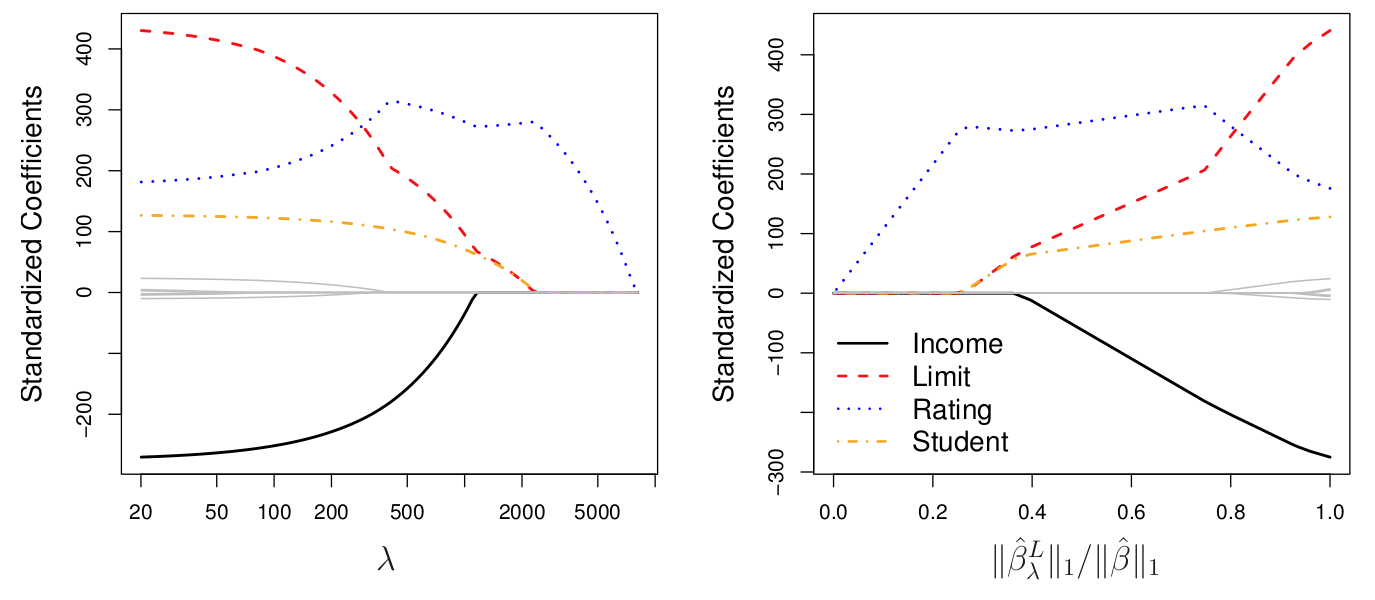
\includegraphics[width = \textwidth]{Fig6-6}
\end{columns}


\InstructorNotes{Also, find best choice of $\lambda$ or $s$ using CV}

\end{frame}
%--- Next Frame ---%


\begin{frame}[t]{Linear transformation of predictors }

\begin{columns}
\column{.45\textwidth}
\centering
\textbf{Original Predictors:}
\begin{equation*}
	X_1,\cdots,X_p
\end{equation*}
\textbf{New Predictors:}
\begin{equation*}
	Z_1,\cdots,Z_M
\end{equation*}
\begin{equation*}
	Z_m = \sum_{j=1}^p \phi_{jm}X_j
\end{equation*}
\column{.45\textwidth}
\centering
\textbf{The goal:}
\begin{itemize}
\item Find good $\phi$'s (PCA)
\item Fit regression model on $Z_i$'s using least squares (PLS)
\begin{equation*}
	y_i = \theta_0 + \sum_{m=1}^M \theta_m z_{im} + \e_i
\end{equation*}
\item Hope that lower dimensions means less overfitting
% \item Remember that interpretation not the same as shrinkage/subset selection of variables
\end{itemize}
\end{columns}

\end{frame}
%--- Next Frame ---%
% \begin{frame}[c]{PCA - First PC}

% \begin{columns}
% \column{.4\textwidth}
% \centering
% 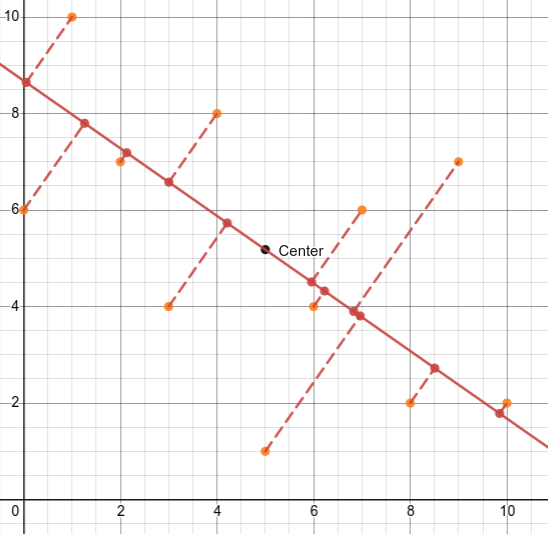
\includegraphics[width = \textwidth, align = c]{PCA-ex-A}
% Projection has high variance
% \column{.4\textwidth}
% \centering
% 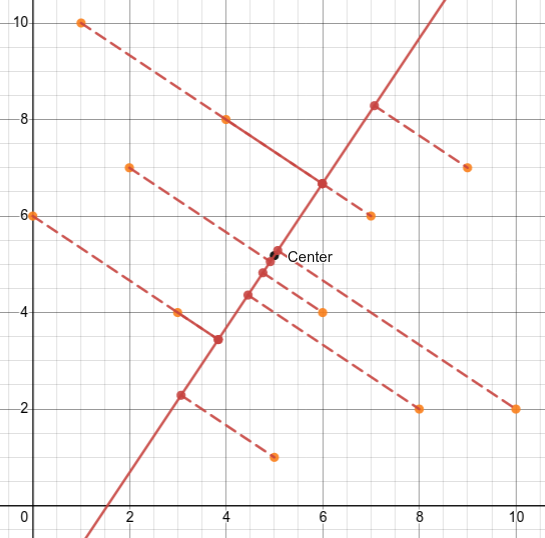
\includegraphics[width = \textwidth, align = c]{PCA-ex-B}
% Projection has low(er) variance

% \end{columns}

% \end{frame}
%--- Next Frame ---%
\begin{frame}[t]{PCA - First PC}
	\begin{columns}
	\column{.24\textwidth}
	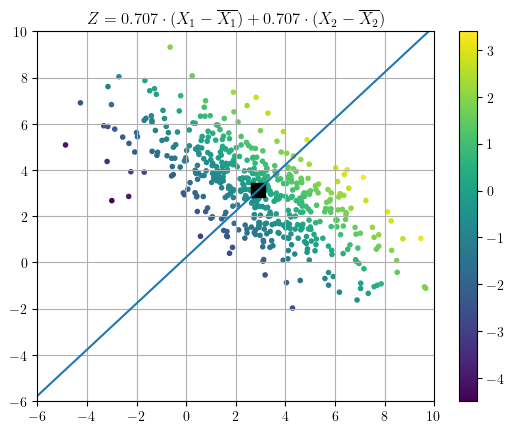
\includegraphics[align = c, width = \textwidth]{DimReduction_Projection_Example2_78.png} 
	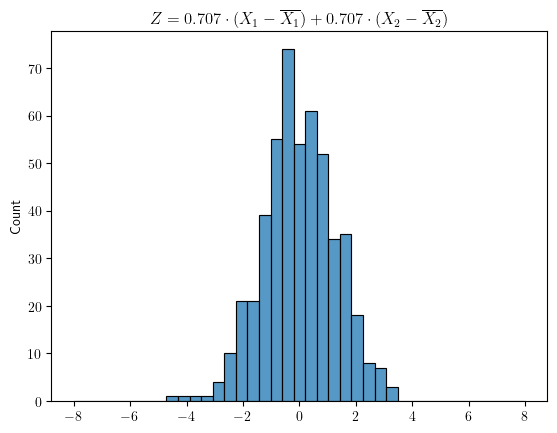
\includegraphics[align = c, width = \textwidth]{DimReduction_Projection_Example2_hist78.png} 
	\column{.24\textwidth}
	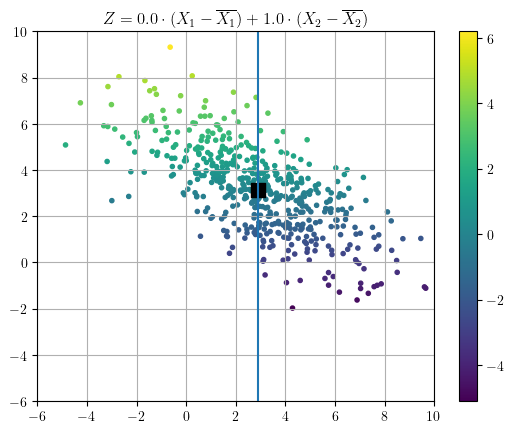
\includegraphics[align = c, width = \textwidth]{DimReduction_Projection_Example2_157.png} 
	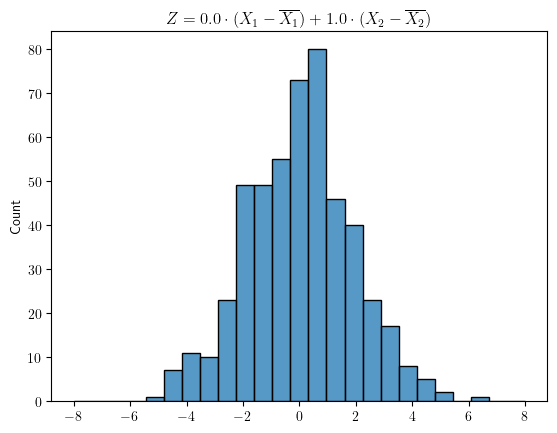
\includegraphics[align = c, width = \textwidth]{DimReduction_Projection_Example2_hist157.png} 
	
	\column{.24\textwidth}
	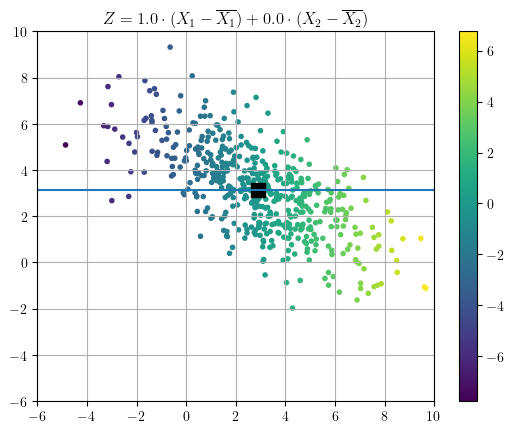
\includegraphics[align = c, width = \textwidth]{DimReduction_Projection_Example2_0.png} 
	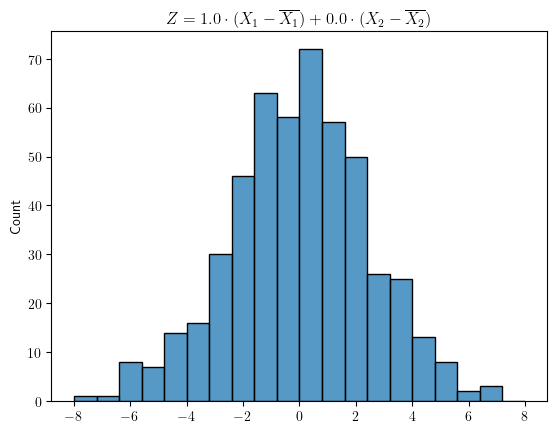
\includegraphics[align = c, width = \textwidth]{DimReduction_Projection_Example2_hist0.png} 

	\column{.24\textwidth}
	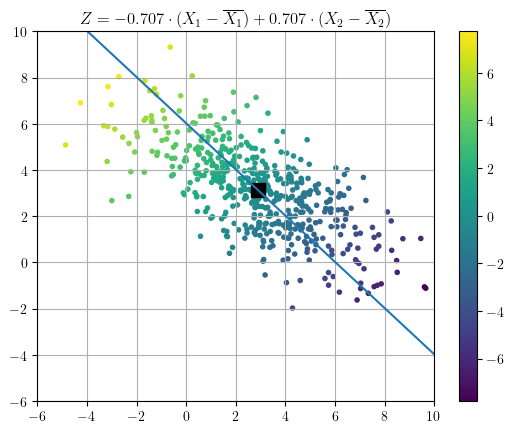
\includegraphics[align = c, width = \textwidth]{DimReduction_Projection_Example2_235.png} 
	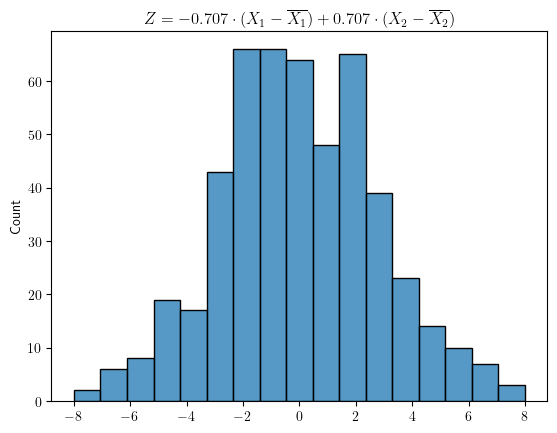
\includegraphics[align = c, width = \textwidth]{DimReduction_Projection_Example2_hist235.png} 


	\end{columns}

	\InstructorNotes{higher variance of projection on the further right pic}
	\end{frame}
	%--- Next Frame ---%

\begin{frame}[c]{Projection onto first PC}

	\centering
	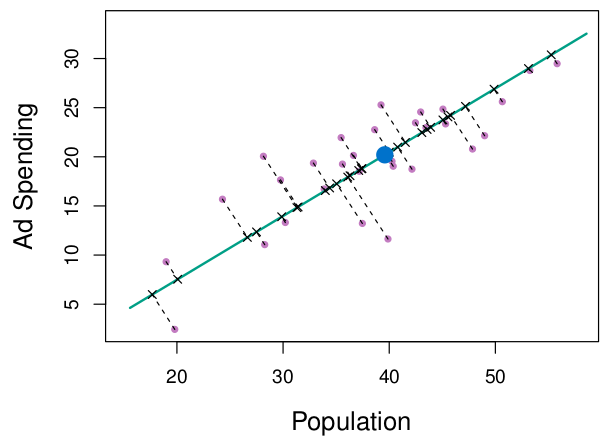
\includegraphics[width =.6 \textwidth, align = c]{Fig6-15a}

	\begin{equation*}
		Z_1 = 0.839 \cdot (\texttt{pop} - \overline{\texttt{pop}}) + 0.544 \cdot (\texttt{ad} - \overline{\texttt{ad}})
	\end{equation*}
	\InstructorNotes{$\phi_{11} = 0.839$ and $\phi_{21} = 0.544$ are the principal component loadings. Blue dot is $(\overline{pop},\overline{ad})$ }


\end{frame}
%--- Next Frame ---%




\begin{frame}[t]{Drawing points in PC space}

\centering
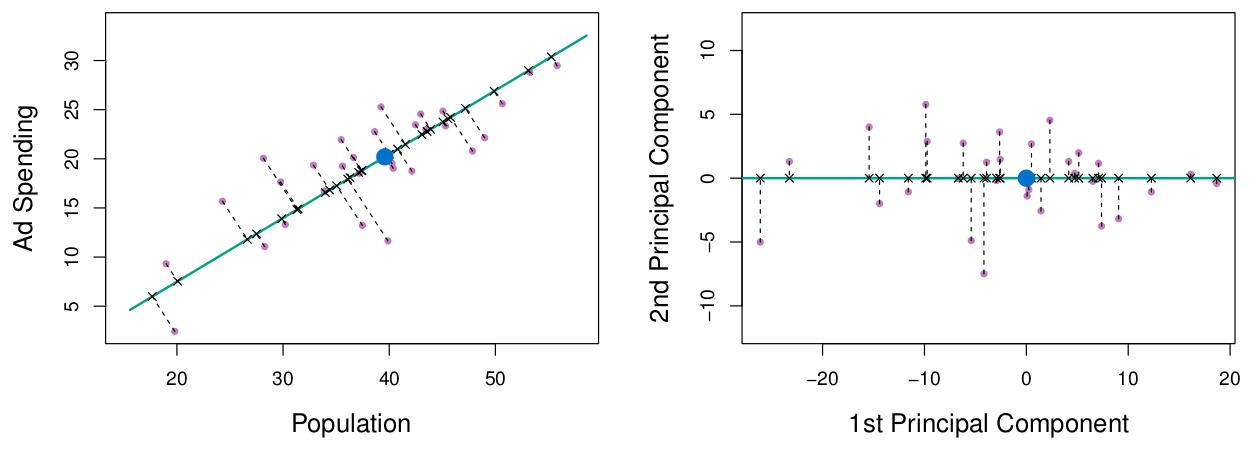
\includegraphics[width = .8\textwidth, align = c]{Fig6-15}
\begin{columns}
\column{.45\textwidth}
\centering
\column{.45\textwidth}
\centering

\end{columns}

\end{frame}
%--- Next Frame ---%

% \begin{frame}[c]{Principal Components Regression (PCR)}

% \begin{columns}
% \column{.4\textwidth}
% \centering
% \begin{itemize}
% 	\item Take new features $Z_i$
% 	\item Run regression
% 	\item Maybe do CV for a bunch of choices of $M$ (where $M = $ number of $Z_i$ features used) to pick a best $M$
% \end{itemize}
% \column{.5\textwidth}
% \centering
% \InstructorList{
%   \item Note that you can't directly use coefficients learned to interpret original inputs 
%   \item Each PC is a linear combination of the originals, so can go backwards to figure out whaat the coefficients would have been, see left figure 
% }

% \end{columns}

% \end{frame}
%--- Next Frame ---%
\begin{frame}[t]{Interpretation of PCR coefficients }
\begin{columns}
\column{.35\textwidth}
\centering
\textbf{Original Predictors:}
\begin{equation*}
	X_1,\cdots,X_p
\end{equation*}
\textbf{New Predictors:}
\begin{equation*}
	Z_1,\cdots,Z_M
\end{equation*}
\begin{equation*}
	Z_m = \sum_{j=1}^p \phi_{jm}X_j
\end{equation*}
\textbf{Learned model:}
\begin{equation*}
	y = \theta_0 + \theta_1 Z_1 + \cdots + \theta_M Z_M
\end{equation*}



\column{.55\textwidth}
\centering
\footnotesize
\InstructorList{
	\item Do example showing that coefficients of $Z_i$ can't be used to say anything about $X_i$'s 
	\item $p=3, M=2$
	\item 
	$\phi = \begin{pmatrix}
	1 & -1  \\
	3 & 1/2 \\
	0 & 1/2
	\end{pmatrix}$
	\item  Learned model $ y = 2 Z_1 - Z_2$
	\item $y = 2(X_1+3X_2 + 0X_3) - (-X_1 + \tfrac{1}{2} X_2 +  \tfrac{1}{2} X_3  )$
	\item $= 3X_1 + 2.5 X_2 - 0.5 X_3 $
	\item Conclusion: can't directly use coefficients learned to interpret original inputs! 
  \item Each PC is a linear combination of the originals, so can go backwards to figure out whaat the coefficients would have been, see left figure 
}
\end{columns}
\end{frame}
%--- Next Frame ---%
\begin{frame}[c]{Bias variance trade-off}
Example with simulated data: $n=50$ observations of $p=45$ predictors\\
$Y$ is a function of \textbf{all predictors}
\begin{columns}
\column{.45\textwidth}
\centering
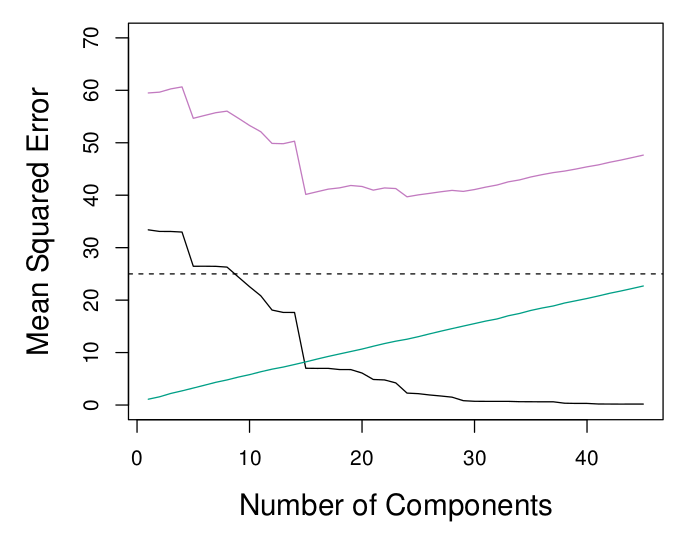
\includegraphics[width = \textwidth, align = c]{Fig6-18a}
\column{.45\textwidth}
\centering
\InstructorList{
\item Right side is usual least squares estimate
\item Even better improvement using PCR than previous
\item note the chnage in $y$-axis values
}
\end{columns}

\end{frame}
%--- Next Frame ---%
\begin{frame}[c]{Bias variance trade-off}
Example with simulated data: $n=50$ observations of $p=45$ predictors\\
$Y$ is a function of \textbf{2 predictors}
\begin{columns}
\column{.45\textwidth}
\centering
\InstructorList{
\item Right side is usual least squares estimate
\item Typical U shape for Test MSE
\item PCR with good choice of number of components improvement over plain least squares
}
\column{.45\textwidth}
\centering
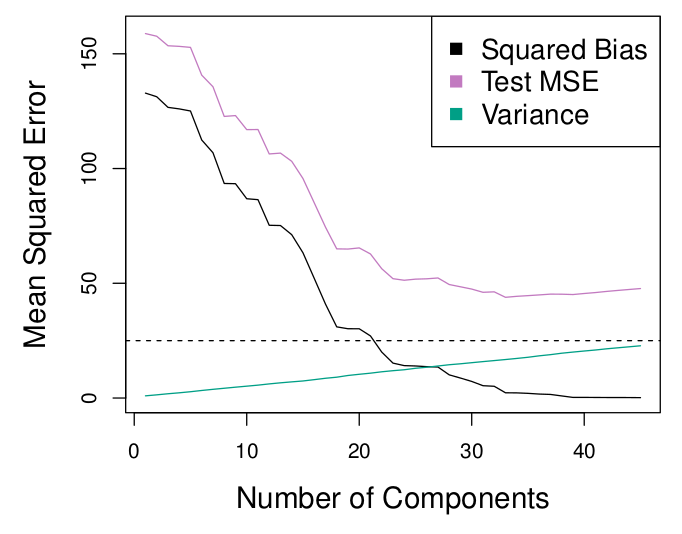
\includegraphics[width = \textwidth, align = c]{Fig6-18b}
\end{columns}

\end{frame}
%--- Next Frame ---%

% \begin{frame}[c]{Comparison to results on shrinkage}

% \begin{columns}
% \column{.45\textwidth}
% \centering
% $Y$ is a function of all predictors
% 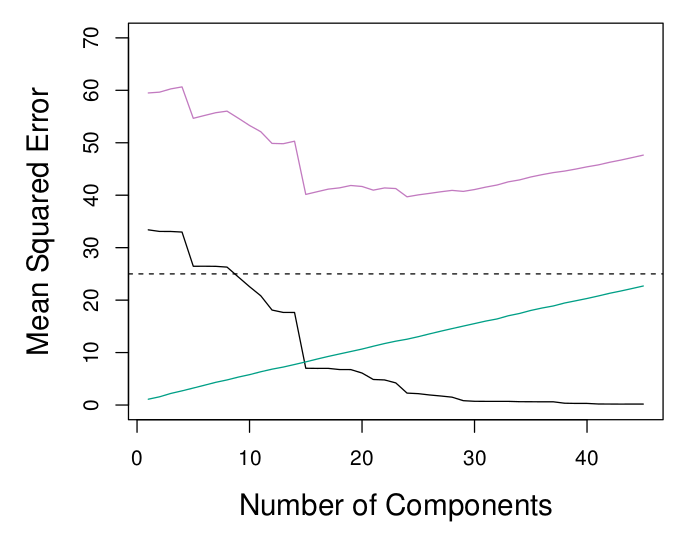
\includegraphics[width = .5\textwidth, align = c]{Fig6-18a}
% 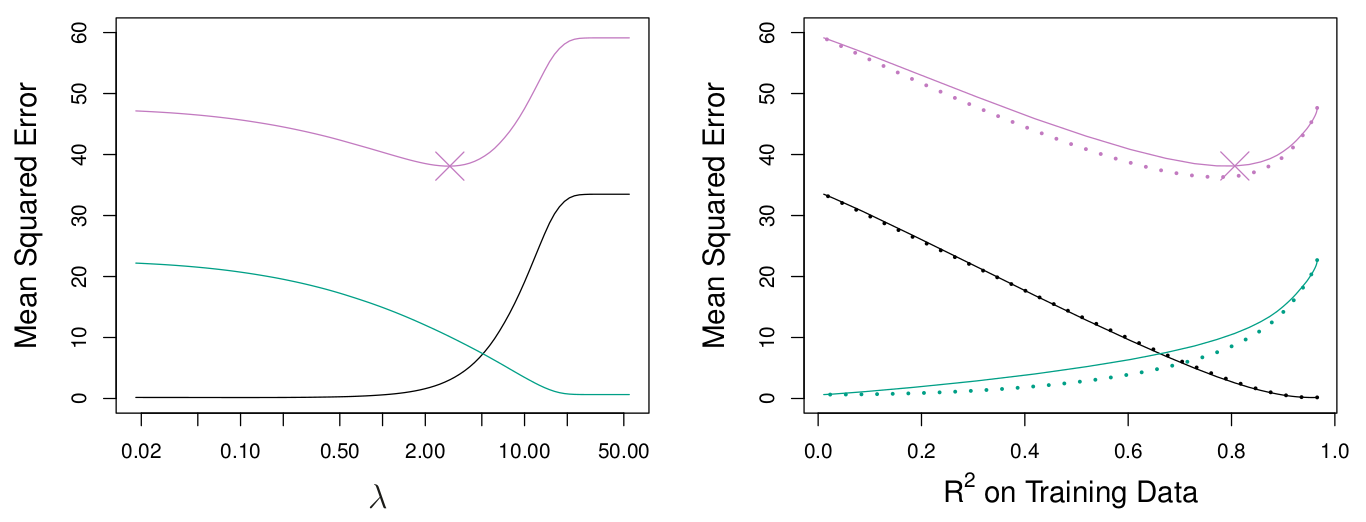
\includegraphics[width = \textwidth, align = c]{Fig6-8}
% \column{.45\textwidth}
% \centering
% $Y$ is a function of 2 predictors
% 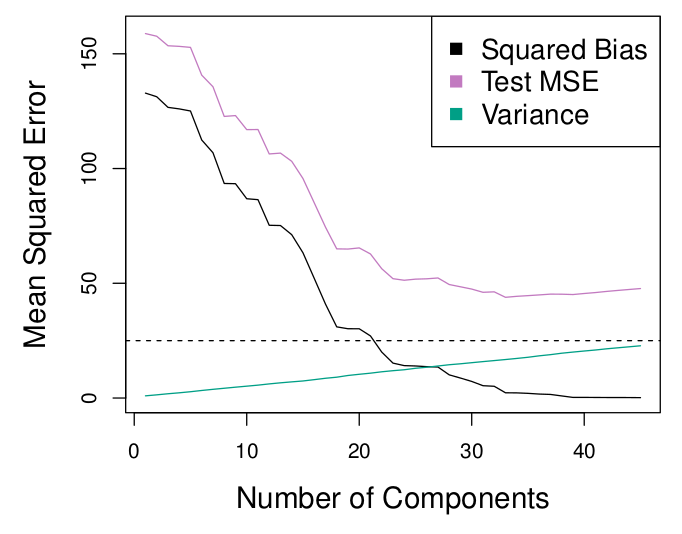
\includegraphics[width = .5\textwidth, align = c]{Fig6-18b}
% 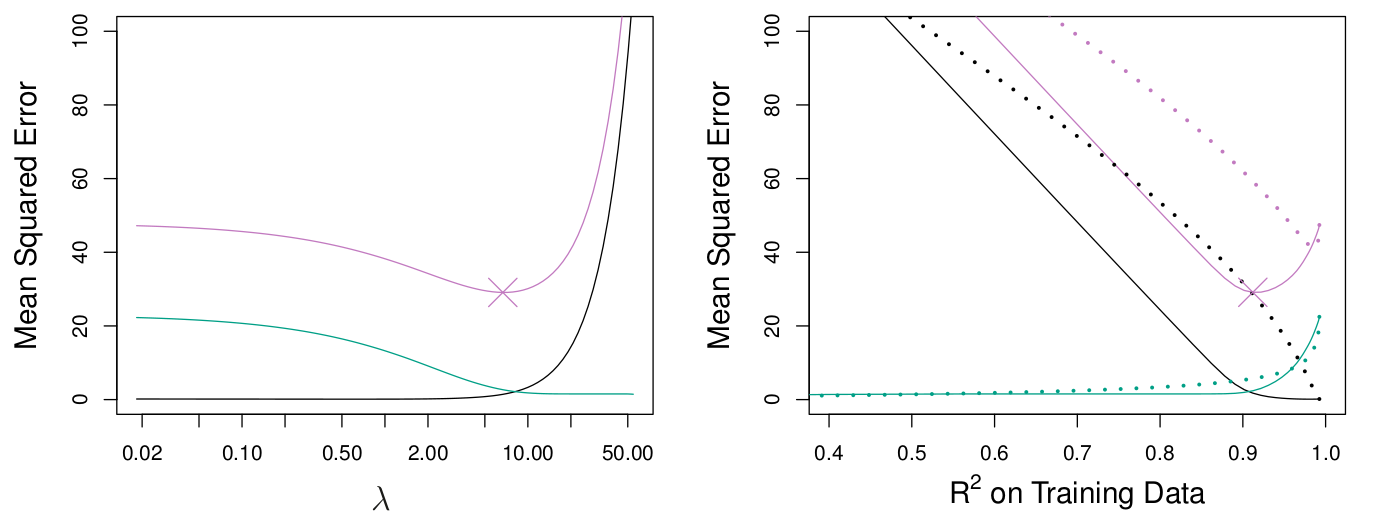
\includegraphics[width = \textwidth, align = c]{Fig6-9}

% \end{columns}
% \InstructorNotes{Shrinkage does better}
% \end{frame}
%--- Next Frame ---%
% \begin{frame}[c]{Picking $M$}

% \begin{columns}
% \column{.75\textwidth}
% \centering
% 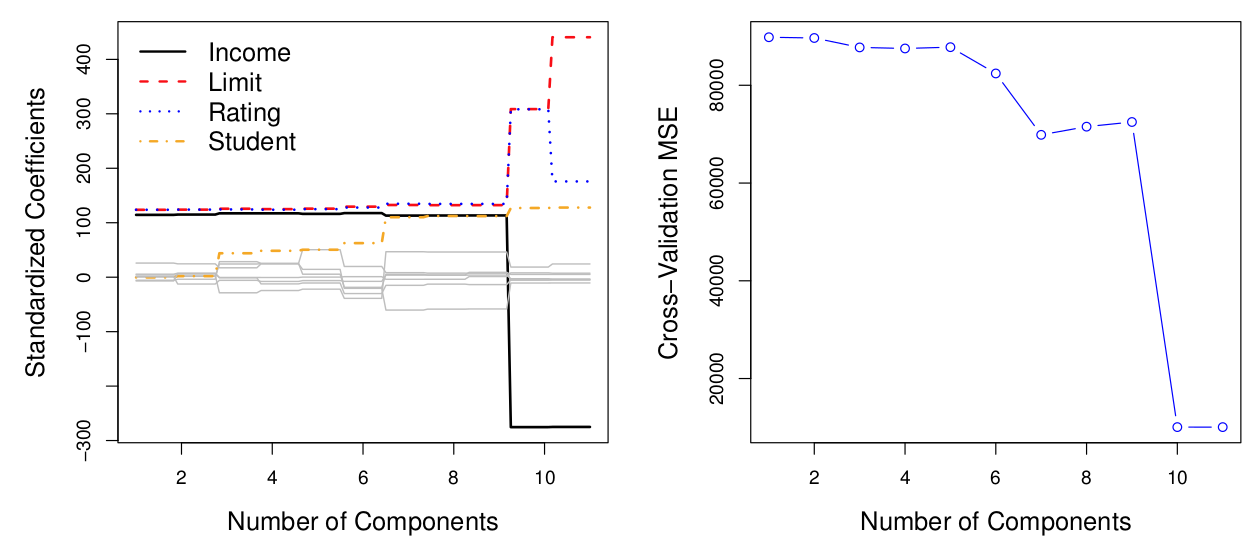
\includegraphics[width = \textwidth]{Fig6-20}
% % \column{.45\textwidth}
% % \centering

% \end{columns}
% \InstructorList{
% \item Credit data set
% \item Major drop in MSE at 10 compoentns, so barely a savings with the original 11 variables
% }

% \end{frame}
%--- Next Frame ---%
\begin{frame}[c]{Properties of PCR}

\begin{columns}
\column{.45\textwidth}
\centering
\InstructorList{
\item Note better in previous example because lots of PCs needed
\item It does better when info contained in the first few PCs
\item Number of PCs to use can be picked with CV
\item Standardization needed to make sure big data values don't skew the results
}
\column{.45\textwidth}
\centering
\InstructorList{
\item Not a feature selection method because we don't get a subset of features, we get a collection of linear combos of features
}
\end{columns}

\end{frame}
%--- Next Frame ---%




%--- Next Frame ---%
	

% {
% \setbeamercolor{background canvas}{bg=Apricot!25}
% \begin{frame}[t]{Figuring out the original model from the PC model }
% \begin{columns}
% \column{.45\textwidth}
% \centering
% \begin{itemize}
% 	\item 
% We have three input variables $X_1, X_2, X_3$
% \item 
% We have two PCs, 
% \begin{align*}
% 	Z_1 &= 0.266 \cdot X_1 -0.077 \cdot X_2 + 0.961 \cdot X_3\\ 
% 	Z_2 &= 0.968 \cdot X_1 +0.136 \cdot X_2 + -0.254 \cdot X_3 
% \end{align*}
% \item Using linear regression, we learn the model 
% \begin{equation*}
% 	Y = -3 + 2Z_1 -4 Z_2.
% \end{equation*}
% \item What are the coefficients for the model in terms of the $X_i$'s? 
% \end{itemize}
% \column{.45\textwidth}
% \centering
% \InstructorNotes{
% 	\tiny
%   \begin{align*}
% 	Y &= -3 + 2Z_1 -4 Z_2\\
% 	&= -3 + 2(0.266 \cdot X_1 -0.077 \cdot X_2 + 0.961 \cdot X_3)\\
% 	& \qquad -4(0.968 \cdot X_1 +0.136 \cdot X_2 + -0.254 \cdot X_3 )\\
% 	&= -3 - 3.34 X_1 - 0.698 X_2 + 2.938 X_3
%   \end{align*}
% }

% \end{columns}
% \end{frame}
% }
% %--- Next Frame ---%
% \begin{frame}[t]{Example on Credit dataset}
% \begin{columns}
% \column{.6\textwidth}
% 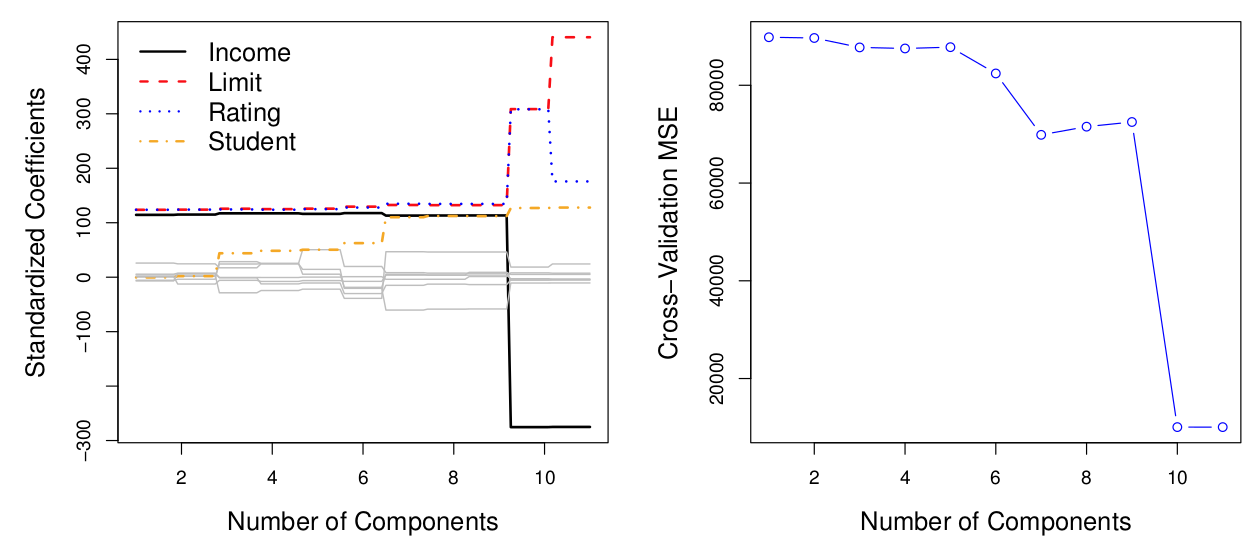
\includegraphics[width = \textwidth, align = c]{Fig6-20}
% \centering
% % \column{.45\textwidth}
% \centering
% \end{columns}

% \InstructorList{
%   \item Not a subset selection method because all $X_i$'s still seen 
%   \item Book says you can view ridge regression as a continuous version of PCR
%   \item In this example, would likely pick $M=10$ components.  Since had 11 originally, not much reduction
% }

% \end{frame}
%--- Next Frame ---%

%=================
\section{Partial Least Squares (PLS)}
%=================



\begin{frame}[t]{Supervised alternative}

\begin{columns}
\column{.45\textwidth}
\centering
PCR: Non-supervised
\InstructorList{
\item No input from the $Y$ values before learning the PCs.
\item No guarantee that directions that explain $X$s help to predict the $Y$s
}
\column{.45\textwidth}
\centering
Partial Least Squares (PLS):
\InstructorList{
	\item Identify new features $Z_1,\cdots,Z_M$ linear combos of original where quality measure involves $Y$
	\item Fit linear model using least squares on these $M$ features
}
\end{columns}

\end{frame}
%--- Next Frame ---%

\begin{frame}[t]{First direction $Z_1$ for Partial Least Squares (PLS)}

\begin{columns}
\column{.45\textwidth}
\centering
\begin{itemize}
	\item Set $\phi_{j1}$ equal to the coefficient from simple linear regression of $Y$ onto $X_j$
	\InstructorNotes{ \footnotesize
 This means we do $p$ linear regressions, not that we take the multivariable linear regression coefficients
	}
	\item The first direction is
	\begin{equation*}
		Z_1 = \sum_{j=1}^p \phi_{j1}X_j
	\end{equation*}
\end{itemize}

\footnotesize
\InstructorList{
\item
PLS places highest weight on variables most strongly related to the response
\item In example, PLS chooses direction less change in ad direction than pop relative to PCA
\item Implies pop more highly correlated with response than ad
}

\column{.45\textwidth}
\centering
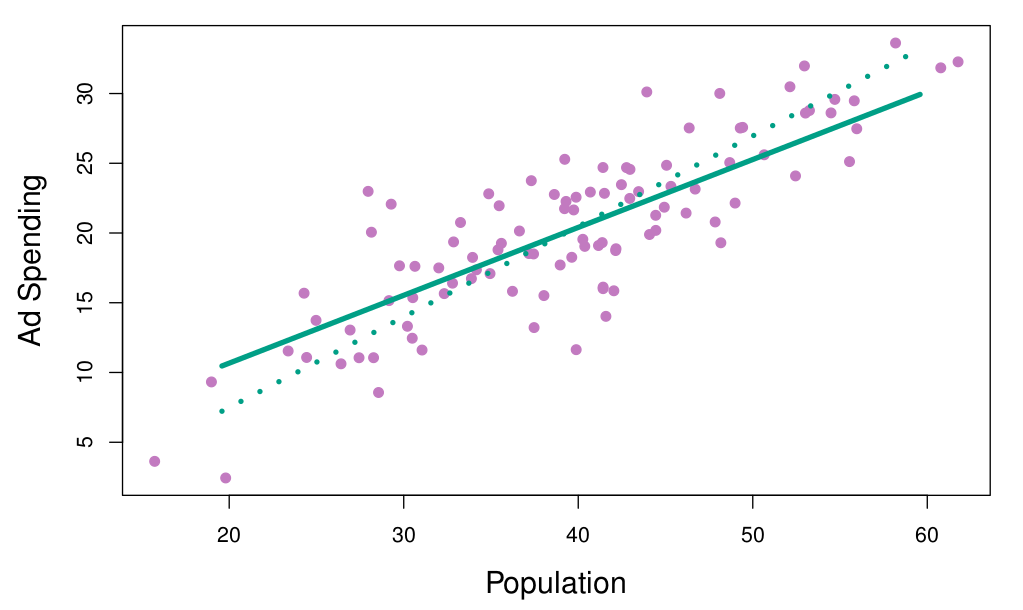
\includegraphics[width = \textwidth]{Fig6-21}
Ex.~Prediction of $Y=$Sales (not shown) on $X_1=$Population and $X_2=$Ad Spending
\begin{itemize}
	\item Solid green: First PLS direction
	\item Dashed: First PC direction
\end{itemize}
\end{columns}

\end{frame}
%--- Next Frame ---%

\begin{frame}[c]{Second (and more) PLS directions}

\begin{columns}
\column{.45\textwidth}
\centering
\begin{itemize}
	\item Regress each variable on $Z_1$ and take residuals
	\InstructorNotes{This is the remaining info not explained by first PLS direction}
	\item Compute $Z_2$ using \textit{orthogonalized data} same as for $Z_1$
\end{itemize}
\InstructorList{
\item Number $M$ can be picked using CV after standardizing predictors
\item Mixed bag in terms of results..... in practice often performs no better than ridge or PCR
}
\column{.45\textwidth}
\centering

\end{columns}

\end{frame}
%--- Next Frame ---%

{
\setbeamercolor{background canvas}{bg=Apricot!25}
\begin{frame}[t]{Code example on hitters data}
\begin{columns}
\column{.45\textwidth}
\centering
\column{.45\textwidth}
\centering
\end{columns}
\end{frame}
}
%--- Next Frame ---%


% \begin{frame}[t]{First direction $Z_1$ for Partial Least Squares (PLS)}

% 	\begin{columns}
% 	\column{.45\textwidth}
% 	\centering
% 	\begin{itemize}
% 		\item Set $\phi_{j1}$ equal to the coefficient from simple linear regression of $Y$ onto $X_j$
% 		\InstructorNotes{ \footnotesize
% 	 This means we do $p$ linear regressions, not that we take the multivariable linear regression coefficients
% 		}
% 		\item The first direction is
% 		\begin{equation*}
% 			Z_1 = \sum_{j=1}^p \phi_{j1}X_j
% 		\end{equation*}
% 	\end{itemize}
	
% 	\footnotesize
% 	\InstructorList{
% 	\item
% 	PLS places highest weight on variables most strongly related to the response
% 	\item In example, PLS chooses direction less change in ad direction than pop relative to PCA
% 	\item Implies pop more highly correlated with response than ad
% 	}
	
% 	\column{.45\textwidth}
% 	\centering
% 	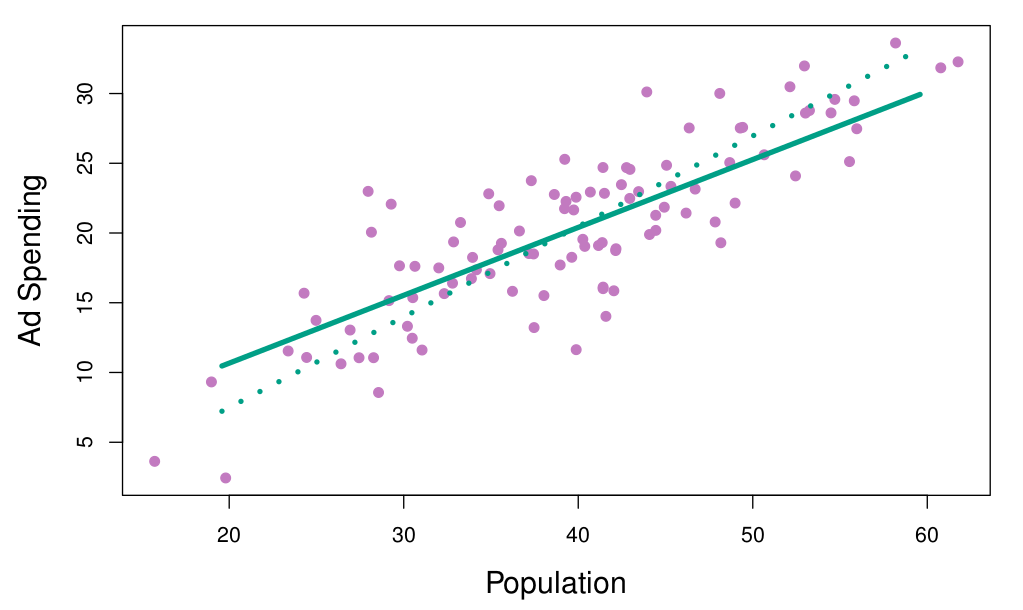
\includegraphics[width = \textwidth]{Fig6-21}
% 	Ex.~Prediction of $Y=$Sales (not shown) on $X_1=$Population and $X_2=$Ad Spending
% 	\begin{itemize}
% 		\item Solid green: First PLS direction
% 		\item Dashed: First PC direction
% 	\end{itemize}
% 	\end{columns}
	
% 	\end{frame}
% 	%--- Next Frame ---%
	
% 	\begin{frame}[c]{Second (and more) PLS directions}
	
% 	\begin{columns}
% 	\column{.45\textwidth}
% 	\centering
% 	\begin{itemize}
% 		\item Regress each variable on $Z_1$ and take residuals
% 		\InstructorNotes{This is the remaining info not explained by first PLS direction}
% 		\item Compute $Z_2$ using \textit{orthogonalized data} same as for $Z_1$
% 	\end{itemize}
% 	\InstructorList{
% 	\item Number $M$ can be picked using CV after standardizing predictors
% 	\item Mixed bag in terms of results..... in practice often performs no better than ridge or PCR
% 	}
% 	\column{.45\textwidth}
% 	\centering
	
% 	\end{columns}
	
% 	\end{frame}
% 	%--- Next Frame ---%
	
	
	
	\begin{frame}[c]{PCR vs PLS}
	
	\begin{columns}
	\column{.45\textwidth}
	\centering
	\textbf{PCR}
	\begin{itemize}
		\item Unsupervised dimensionality reduction $+$ linear regression
		\item Choose component $Z_1$ in the direction of most variance using only $X_i$'s information
		\item Choose $Z_2$ and beyond by the same method after ``getting rid'' of info in the directions already explained
	\end{itemize}
	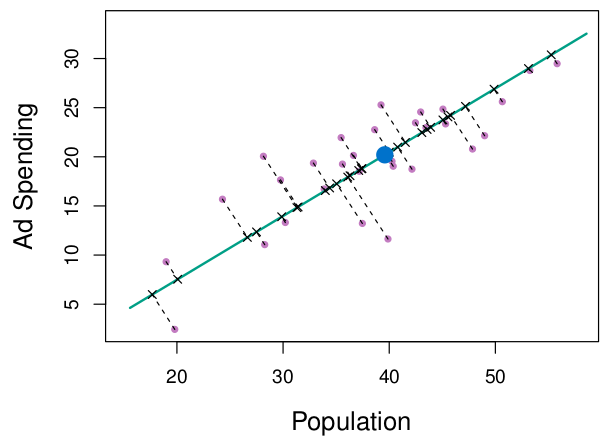
\includegraphics[width = .5\textwidth, align = c]{Fig6-15a}
	
	\column{.45\textwidth}
	\centering
	\textbf{PLS}
	\begin{itemize}
		\item Supervised dimensionality reduction
		\item Choose component $Z_1$ by using simple regression coefficients of each $X_i$ onto $Y$
		\item Choose $Z_2$ and beyond by the same method after ``getting rid'' of info in the directions already explained
		\item Not a particular benefit, so usually default to PCA unless you have a good reason for this
	\end{itemize}
	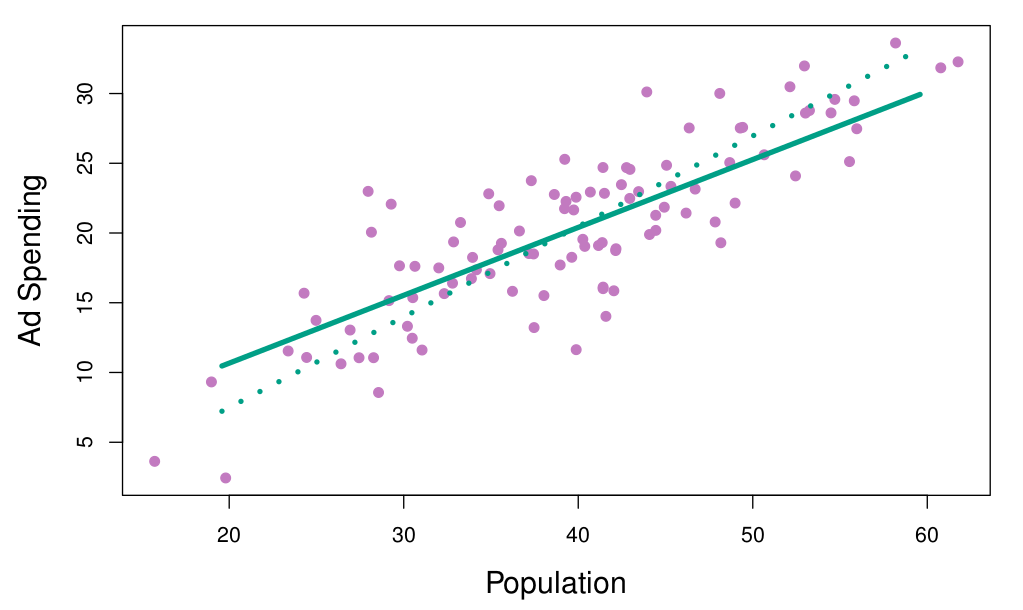
\includegraphics[width = .5\textwidth]{Fig6-21}
	
	\end{columns}
	
	\end{frame}
	%--- Next Frame ---%
	
%==========
\section{Issues in Higher Dimensions}
%==========
\begin{frame}[c]{Goal of this chapter}

\begin{columns}
\column{.45\textwidth}
\centering
% Use something other than least squares to fit:

\InstructorNotes{Classes of methods }
\InstructorList{
\item Subset selection: identify subset of predictors, fit model using least squares on smaller set of variables
\item Shrinkage:
\InstructorList{
\item Estimated coeff are shrunken towards zero relative to the least squares estimate
}
\item Dimension reduction: Project the $p$-dimensional data into $M$-dimensional subspace, $M <p$. Likely after the midterm.
}
\column{.45\textwidth}
\centering

\end{columns}

\end{frame}
%--- Next Frame ---%
\begin{frame}[t]{High-Dimensional Data}

\begin{columns}
\column{.45\textwidth}
\centering
\textbf{Low-Dimensions}

$n \gg p$

\footnotesize
\InstructorList{
\item Low here means $p$ is low, or at least small relative to $n$
\item Can do all the stuff we've talked about so far
\item Historically, this is the data we had to work with
\item e.g. Predict blood pressure on age, sex, BMI. $p=3$ and we have hundreds of thousands of patients to work with
}
\column{.45\textwidth}
\centering
\textbf{High-Dimensions}

$n \ll p$

\footnotesize
\InstructorList{
  \item New technology makes this possible
	\item Predict blood pressure based on single nucleotide polymorphisms (SNPs, individual DNA mutations). $n \approx 200$, $p \approx 500,000$
	\item Search engine bag of words model. Maybe you can access a few hundred people, but each word is scored as present (0) or (1) absent.  Huge number of words
	\item Classical approaches not appropriate since overfitting, bias-variance tradeoff
	\item Issues show up even if $p$ is slightly smaller than $n$
}



\end{columns}

\end{frame}
%--- Next Frame ---%

\begin{frame}[t]{What goes wrong?}
\centering

$n \gg p$ \hspace{1in} $n \approx p$ 

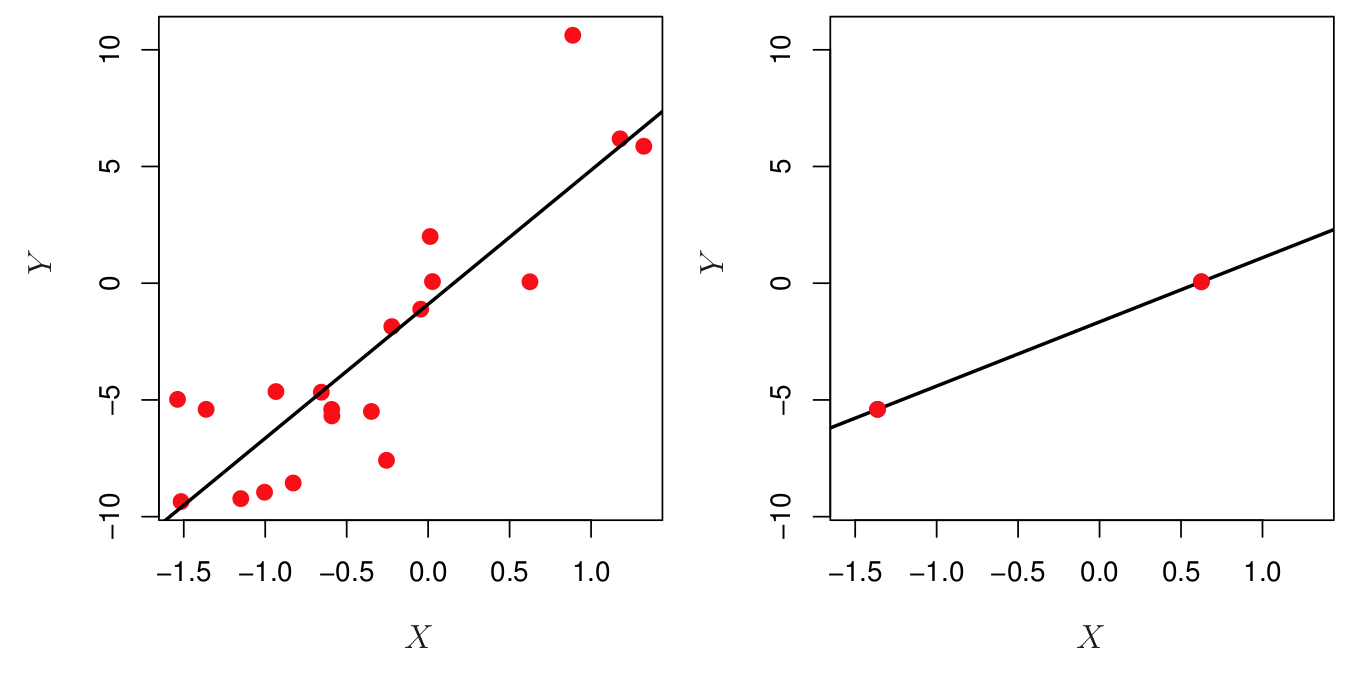
\includegraphics[width = .5\textwidth, align = c]{Fig6-22}
\begin{columns}
\column{.3\textwidth}
\centering


\InstructorList{
  \item $p=1$ feature
	\item $n \gg p$
	\item Not perfect fit, but more reasonable fit
}


\column{.3\textwidth}
\centering
\footnotesize
\InstructorList{
  \item $p=1$ feature
	\item $n =2$ just barely bigger than $p$
	\item Fit will always be perfect
	}
	\column{.35\textwidth}
	\centering
	\footnotesize
	\InstructorList{
	\item If this is 2 samples from the same as the left, result is a pretty bad model
	\item Idea: if $p>n$ or $p \approx n$, then line is too flexible so overfits
}

\end{columns}

\end{frame}
%--- Next Frame ---%
\begin{frame}[t]{More issues with least squares on big $p$}
\begin{columns}
\column{.5\textwidth}
\centering
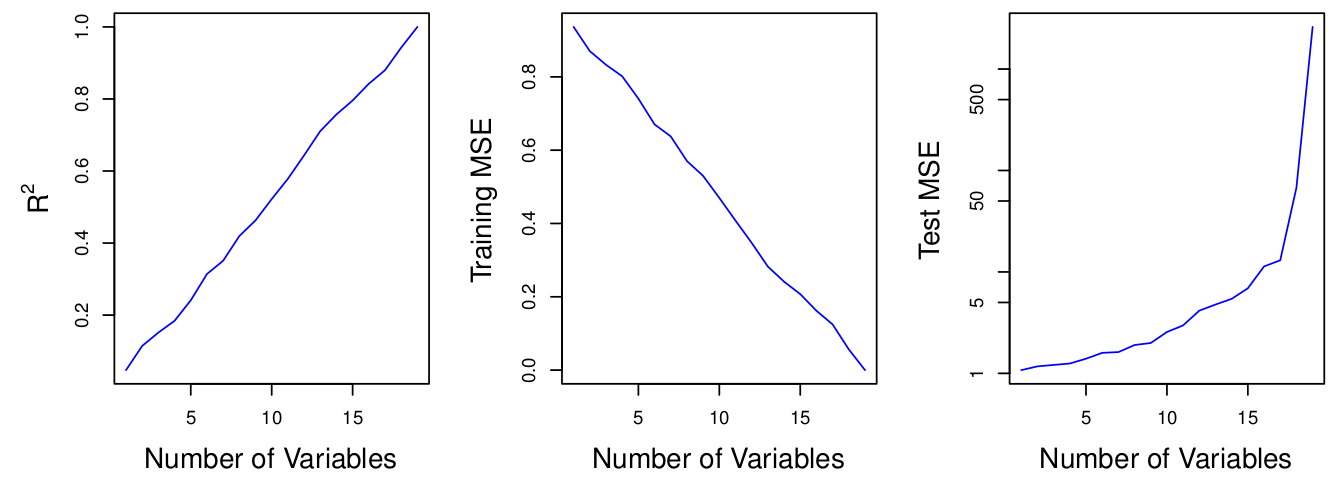
\includegraphics[width = \textwidth, trim = 450 0 0 0, clip]{Fig6-23}

\column{.4\textwidth}
\centering
\begin{itemize}
	\item $n=20$
	\item Regression on $p=1,\cdots,20$
	\item $Y$ completely unrelated to variables
\end{itemize}
\end{columns}


\begin{columns}
\column{.45\textwidth}
\centering

\InstructorList{
  \item Training MSE goes to 0 even though this whole set is garbage
	\item Test MSE gets worse because additional predictors lead to increase in variance of coeff estimates
}

\column{.45\textwidth}
\centering

\footnotesize
\InstructorList{
	\item If you just look at $R^2$ or training MSE, you would suspect that more variables is better
  \item Extra care needed when analyzing data with very large $p$
	\item Like $R^2$, $C_p$, AIC, BIC don't work well in high dimensions.  Cause is $\hat \sigma^2$ is problematic.
}


\end{columns}



\end{frame}
%--- Next Frame ---%
\begin{frame}[t]{The answer to dealing with big $p$}

\centering
\textbf{Be less flexible!}
\begin{columns}
\column{.45\textwidth}
\centering

\InstructorList{
  \item Forward step selection
	\item ridge regression
	\item lasso
	\item principal components regression
}

\column{.45\textwidth}
\centering

\end{columns}


\end{frame}
%--- Next Frame ---%
\begin{frame}[t]{Example with Lasso}


\begin{columns}
\column{.7\textwidth}
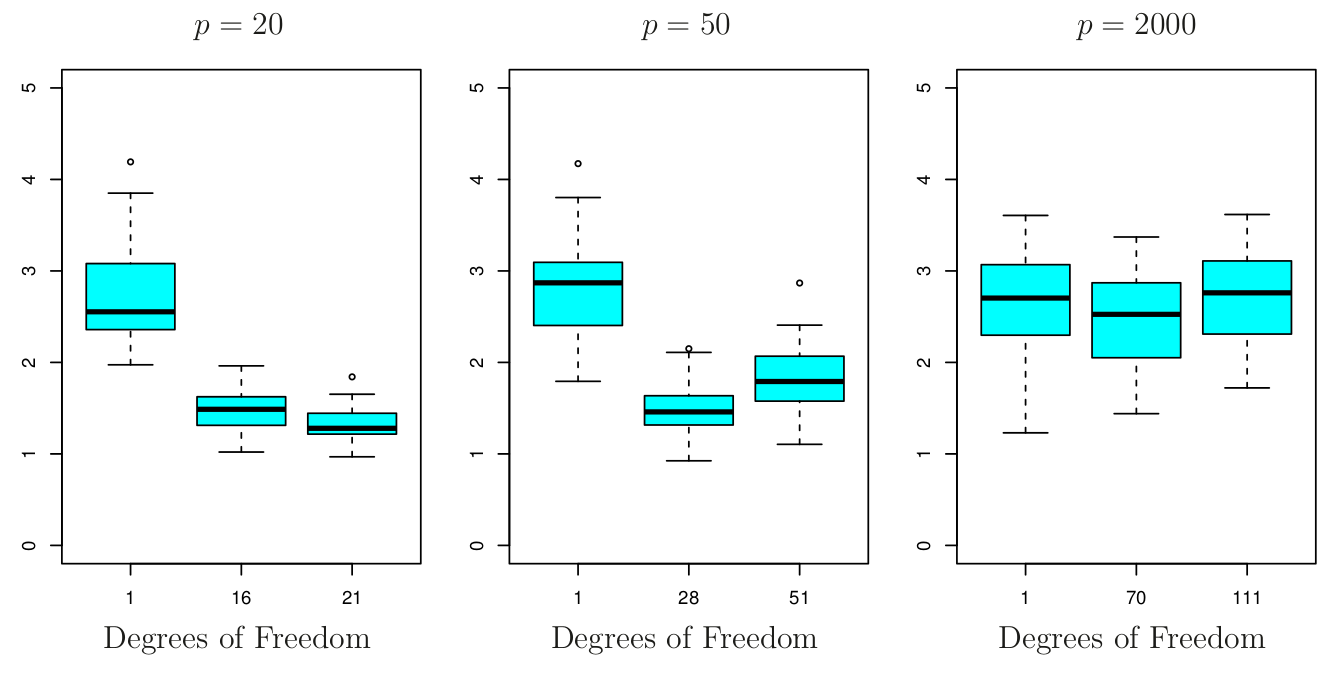
\includegraphics[width = \textwidth]{Fig6-24}
\centering
\column{.29\textwidth}
\begin{itemize}
	\item $n=100$
	\item Boxplots = Test MSE
	\item DF = \# non-zero coeffs \InstructorNotes{Messed with $\lambda$ then reported this}
\end{itemize}

\end{columns}


\begin{columns}
\column{.3\textwidth}
\centering

\footnotesize
\InstructorList{
\item High $\lambda$ means fewer non-zero coeffs means high $\lambda$ is to the left
}

\column{.3\textwidth}
\centering

\footnotesize
\InstructorList{
  \item Small $p$: low val.~set error with $\lambda $ small
	\item $p$ larger means larger $\lambda$ used
}
\column{.3\textwidth}
\centering
\end{columns}



\end{frame}
%--- Next Frame ---%
\begin{frame}[t]{Key points }

\begin{columns}
\column{.45\textwidth}
\centering

\InstructorList{
  \item (1) regularization
or shrinkage plays a key role in high-dimensional problems, \item (2) appropriate
tuning parameter selection is crucial for good predictive performance, and
\item (3) the test error tends to increase as the dimensionality of the problem
(i.e. the number of features or predictors) increases, unless the additional
features are truly associated with the response.
}

\column{.45\textwidth}
\centering

\end{columns}

\end{frame}
%--- Next Frame ---%
\begin{frame}[t]{Curse of dimensionality}
\textit{Phenomena that arise when analyzing and organizing data in high-dimensional spaces that do not occur in low-dimensional settings.}
\begin{columns}
\column{.45\textwidth}
\centering

\InstructorList{
  \item You'd think more variables means better model fit
	\item IN previous example, test MSE doubles as $p$ increases from 20 to 2,000.
}

\column{.45\textwidth}
\centering

\InstructorList{
	\item Addition additional features that are TRULY associated with response will improve fitting model
  \item Adding noise features will result in deterioration
	\item Increase risk of overfitting without upside in test set error
}


\end{columns}

\end{frame}
%--- Next Frame ---%

\begin{frame}[t]{Interpretation in high dimensions}

\begin{columns}
\column{.45\textwidth}
\centering
\textbf{Multi-collinearity:} the concept that the variables in a regression might be correlated with each other


\InstructorList{
\item High dim: any variable in the model can be written as a linear combination of all of the other variables in the model.
}



\column{.45\textwidth}
\centering
\InstructorList{

	\item can never know exactly which variables (if any) truly are predictive of the outcome,
	\item can never identify the best coefficients
for use in the regression.
\item  At most, we can hope to assign large regression
coefficients to variables that are correlated with the variables that truly are
predictive of the outcome.
\item Resulting model is \textit{one of many possible}
}
\end{columns}

\end{frame}
%--- Next Frame ---%
\begin{frame}[t]{Reporting errors in high dimensions}

\begin{columns}
\column{.45\textwidth}
\centering

\InstructorList{
  \item When $p>n$, easy to obtain a useless model that has zero residuals.
	\item Don't use sum of squared errors, p-values, R 2
statistics, or other traditional measures of model fit on the training data as evidence of a good model fit
\item Reporting this fact might mislead others into thinking that a statistically valid and useful model has been obtained
\item in fact this provides absolutely no evidence of a compelling model.
}

\column{.45\textwidth}
\centering

\InstructorList{
  \item Report results on an independent test set, or cross-validation errors.
	\item 	For instance, the MSE or R 2 on an independent test set is a valid measure
	of model fit, but the MSE on the training set certainly is not.
}

\end{columns}

\end{frame}
%--- Next Frame ---%
% \begin{frame}[c]{}

% \begin{columns}
% \column{.45\textwidth}
% \centering
% \Large
% There are three kinds of lies:
% Lies, Damned Lies, and Statistics.
% \column{.45\textwidth}
% \centering
%  $\sim$ Mark Twain (among others), who attributed it to the British prime minister Benjamin Disraeli.
% \end{columns}

% \end{frame}
%--- Next Frame ---%

% \begin{frame}[c]{TL;DR}

% \begin{columns}
% \column{.45\textwidth}
% \centering
% \textbf{PCA}
% \begin{itemize}
% 	\item Unsupervised dimensionality reduction
% 	\item Choose component $Z_1$ in the direction of most variance using only $X_i$'s information
% 	\item Choose $Z_2$ and beyond by the same method after ``getting rid'' of info in the directions already explained
% \end{itemize}
% 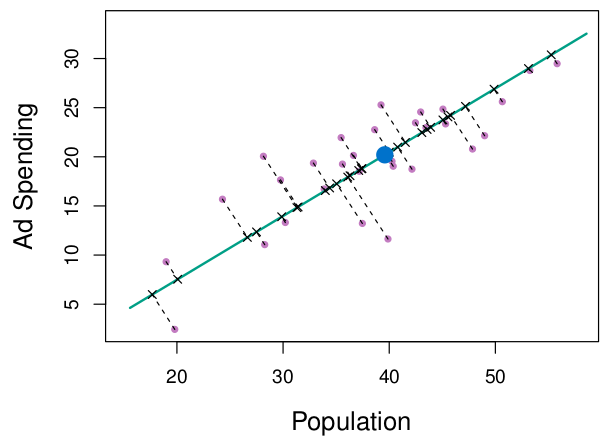
\includegraphics[width = .5\textwidth, align = c]{Fig6-15a}

% \column{.45\textwidth}
% \centering

% \textbf{PCR}
% \begin{itemize}
% 	\item Do PCA on input data 
% 	\item Do Linear Regression on chosen number of PCs. 
% 	\item Warning: Lose interpretability of the coefficients.
% \end{itemize}

% % \begin{itemize}
% % 	\item Supervised dimensionality reduction
% % 	\item Choose component $Z_1$ by using simple regression coefficients of each $X_i$ onto $Y$
% % 	\item Choose $Z_2$ and beyond by the same method after ``getting rid'' of info in the directions already explained
% % 	\item Not a particular benefit, so usually default to PCA unless you have a good reason for this
% % \end{itemize}
% % 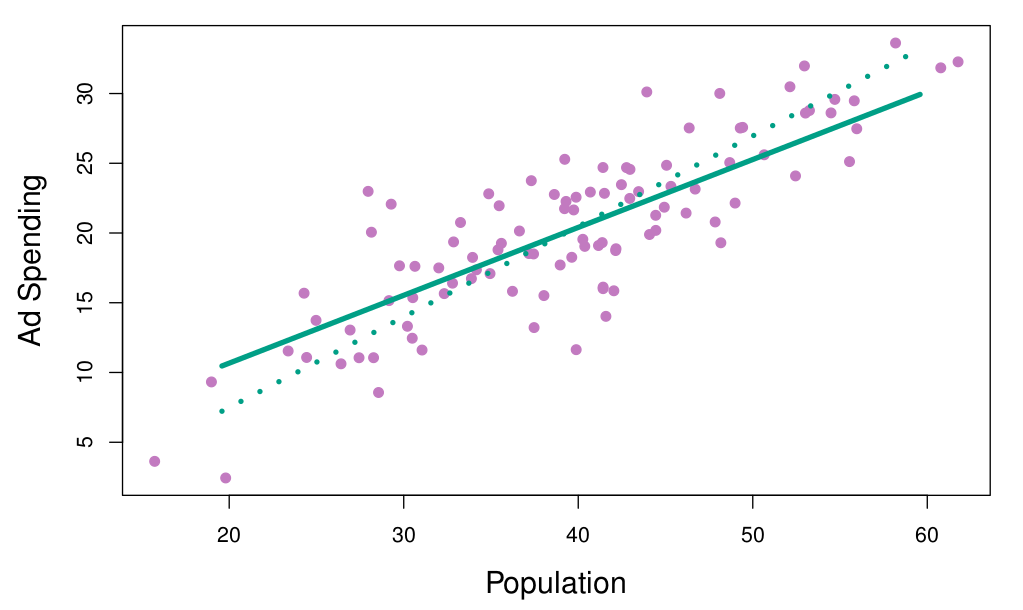
\includegraphics[width = .5\textwidth]{Fig6-21}
% % 
% \end{columns}

% \end{frame}

\begin{frame}[t]{Next time}



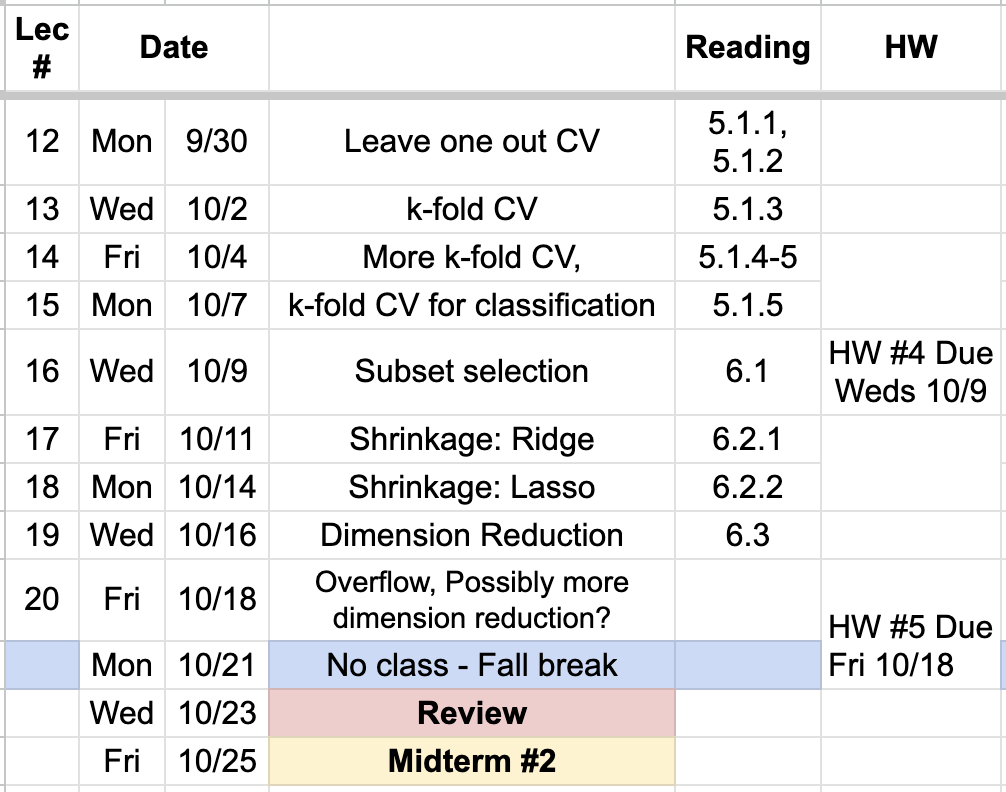
\includegraphics[align = c, width = .5\textwidth]{Day01-Schedule-Test2}

\end{frame}
%--- Next Frame ---%



\end{document}
